\documentclass[aspectratio=169, usenames, dvipsnames]{beamer}

%%%%%
%%%%%
%%%%%     DEFINE THE THEME USED
%%%%%
%%%%%

\usetheme{jc}

%%%%%
%%%%%
%%%%%     LIST OF PACKAGES USED
%%%%%
%%%%%

\graphicspath{{imgs/}}

\usepackage[utf8]{inputenc}
\usepackage[T1]{fontenc}

\usepackage[]{nicefrac}

\usepackage[]{amsmath, amssymb, amsfonts}
\usepackage[]{bm}

\usepackage[]{graphicx}

\usepackage{xcolor}
\usepackage{tikz}
\usetikzlibrary{decorations.pathreplacing}
\usetikzlibrary{backgrounds, matrix}
\usetikzlibrary{arrows, shapes}
\usetikzlibrary{tikzmark}
\usetikzlibrary{calc}
\usetikzlibrary{shadows}
\usetikzlibrary{trees, mindmap}
\usetikzlibrary{shapes.geometric, math, positioning, calc, patterns, angles, quotes}
\usetikzlibrary{patterns.meta,decorations.pathmorphing}

\usepackage{pgfplots}
\pgfplotsset{compat=newest}


\newcommand{\highlight}[2]{\colorbox{#1!17}{$\displaystyle #2$}}
\newcommand{\highlightdark}[2]{\colorbox{#1!47}{$\displaystyle #2$}}
\renewcommand{\highlight}[2]{\colorbox{#1!17}{#2}}
\renewcommand{\highlightdark}[2]{\colorbox{#1!47}{#2}}


\DeclareMathOperator*{\minimize}{minimize~}
\DeclareMathOperator*{\maximize}{maximize~}
\DeclareMathOperator*{\subto}{subject~to~}

%%%%%
%%%%%
%%%%%     INFO ABOUT THE PRESENTATION
%%%%%
%%%%%

\title{On the importance of low-dimensional structures for data-driven modeling}
\author[JC]{Jean-Christophe Loiseau}
\date[]{May, 13\textsuperscript{th} 2022}

%%%%%
%%%%%
%%%%%     PRESENTATION
%%%%%
%%%%%

\begin{document}

\begin{frame}
  \titlepage
\end{frame}


\begin{frame}
  \vfill
  \begin{minipage}{.68\textwidth}
    \begin{itemize}
    \item Maître de Conférences in Fluid Dynamics and Applied Math.

      \bigskip

    \item Machine-learning enthusiast with application to engineering systems.

      \bigskip

    \item Data-efficient models with guarantees of optimality or interpretability.
    \end{itemize}
  \end{minipage}%
  \hfill
  \begin{minipage}{.28\textwidth}
    \includegraphics[width=\textwidth]{myself}
  \end{minipage}

  \vfill
\end{frame}

\begin{frame}
  \vfill

  Given training data $\bm{y}_i = \bm{f}(\bm{x}_i)$ where $\bm{f}$ is unknown, we want to \textbf{learn} a function $\hat{\bm{f}}$ such that

  \bigskip
{\Large
  \[
  \minimize_{\hat{\bm{f}} \in \mathcal{F}} \quad \| \bm{f}(\bm{x}) - \hat{\bm{f}}(\bm{x}) \|
  \]
}

  \bigskip

  where $\mathcal{F}$ is a particular \emph{class} of models.

  \vfill
\end{frame}

\section{A brief overview of SVD}
\begin{frame}
  \sectionpage
\end{frame}

\begin{frame}
  \vfill

  \begin{overprint}

    \onslide<1>
    \Large
    \[
    \bm{A} = {\highlightdark{black!100}{$\bm{U}$}} {\highlightdark{black!100}{$\boldsymbol{\Sigma}$}} {\highlightdark{black!100}{$\bm{V}$}}^T
    \]

    \onslide<2>
    \Large
    \[
    \bm{A} = \tikzmarknode{a} {\highlightdark{red}{$\bm{U}$}} \tikzmarknode{b}{\highlightdark{blue}{$\boldsymbol{\Sigma}$}} \tikzmarknode{c} {\highlightdark{OliveGreen}{$\bm{V}$}}^T
    \]

    \begin{tikzpicture}[overlay, remember picture, >=stealth, nodes={align=left, inner ysep=1pt}, <-]

      \path (a.north) ++ (0, 2em) node[anchor=south east, color=red!67] (U){Basis for $\textrm{colspan}(\bm{A})$};
      \draw [color=red!87] (a.north) |- ([xshift=0.3ex, color=red] U.south west);

      \path (b.south) ++ (0, -2em) node[anchor=north east, color=blue!67] (Sigma){Diagonal matrix};
      \draw [color=blue!87] (b.south) |- ([xshift=-0.3ex, color=blue] Sigma.south west);

      \path (c.north) ++ (0, 2em) node[anchor=south west, color=OliveGreen!67] (V){Basis for $\textrm{rowspan}(\bm{A})$};
      \draw [color=OliveGreen!87] (c.north) |- ([xshift=0.3ex, color=OliveGreen] V.south east);

    \end{tikzpicture}

  \end{overprint}

  \vfill
\end{frame}

\begin{frame}

  \vfill

  \begin{tcolorbox}[
    enhanced,
    coltitle=black,
    coltext=white,
    colback=black,
    title=\textbf{Relation to spectral decomposition},
    frame style tile={width=\paperwidth}{background.jpg}
    ]

  \bigskip

  {\large
  \[
  \begin{bmatrix}
    \bm{0} & \bm{A} \\
    \bm{A}^T & \bm{0}
  \end{bmatrix}
  \begin{bmatrix}
    \bm{u}_i \\ \bm{v}_i
  \end{bmatrix}
  =
  \sigma_i
  \begin{bmatrix}
    \bm{u}_i \\ \bm{v}_i
  \end{bmatrix}
  \]
  }

  \bigskip

  Generalization of the \emph{eigenvalue decomposition} to \textbf{non-square matrices} by E. Beltrami (1873) and C. Jordan (1874).
  The first efficient numerical algorithm was developed by G.\ Golub \emph{et al.} in the late 1960s.

  \end{tcolorbox}
  \vfill

\end{frame}

{
  \setbeamercolor*{background canvas}{bg=white}

  \begin{frame}
    \vfill
    \centering

    \vfill
  \end{frame}
}

\begin{frame}{Ordinary least-squares}
  \vfill
  \begin{minipage}{.48\textwidth}
    \Large
    \[
    y = a x + b
    \]
  \end{minipage}%
  \hfill
  \begin{minipage}{.48\textwidth}
    \centering
    \begin{tikzpicture}[>=stealth]
      \begin{axis}[
          xmin=0, xmax=2,
          ymin=1.5, ymax=4.5,
          xlabel={$x$}, ylabel={$y$},
          width=\textwidth,
          height=.66\textheight,
          axis lines = middle,
          x label style={at={(axis description cs:1, -0.025)}, anchor=north},
          y label style={at={(axis description cs:-0.025, 1)},  anchor=east},
          ytick style={draw=none},
          yticklabels=\empty,
          xtick style={draw=none},
          xticklabels=\empty,
        ]

        % --> Plot singular spectrum.
        \addplot[ultra thick, orange, smooth, only marks, mark size=1.5pt] table[x=x, y=y]{data/ls_data.dat};

      \end{axis}
    \end{tikzpicture}
  \end{minipage}
  \vfill
\end{frame}


\begin{frame}{Ordinary least-squares}
  \vfill
  \begin{minipage}{.48\textwidth}
      \large
      \[
      \minimize_{a, b} \sum_{i=1}^N \left( y_i - a x_i - b \right)^2
      \]
  \end{minipage}%
  \hfill
  \begin{minipage}{.48\textwidth}
    \centering
    \begin{tikzpicture}[>=stealth]
      \begin{axis}[
          xmin=0, xmax=2,
          ymin=1.5, ymax=4.5,
          xlabel={$x$}, ylabel={$y$},
          width=\textwidth,
          height=.66\textheight,
          axis lines = middle,
          x label style={at={(axis description cs:1, -0.025)}, anchor=north},
          y label style={at={(axis description cs:-0.025, 1)},  anchor=east},
          ytick style={draw=none},
          yticklabels=\empty,
          xtick style={draw=none},
          xticklabels=\empty,
        ]

        % --> Plot singular spectrum.
        \addplot[ultra thick, orange, smooth, only marks, mark size=1.5pt] table[x=x, y=y]{data/ls_data.dat};

        \addplot[domain=0.4:1.6, white, ultra thick] {1.01893789 + 1.94042227*x};
      \end{axis}
    \end{tikzpicture}
  \end{minipage}
  \vfill
\end{frame}

\begin{frame}{Ordinary least-squares}
  \vfill
  \begin{minipage}{.48\textwidth}
      \large
      \[
      \minimize_{\bm{x}} \| \bm{Ax} - \bm{b} \|_2^2
      \]
  \end{minipage}%
  \hfill
  \begin{minipage}{.48\textwidth}
    \centering
    \begin{tikzpicture}[>=stealth]
      \begin{axis}[
          xmin=0, xmax=2,
          ymin=1.5, ymax=4.5,
          xlabel={$x$}, ylabel={$y$},
          width=\textwidth,
          height=.66\textheight,
          axis lines = middle,
          x label style={at={(axis description cs:1, -0.025)}, anchor=north},
          y label style={at={(axis description cs:-0.025, 1)},  anchor=east},
          ytick style={draw=none},
          yticklabels=\empty,
          xtick style={draw=none},
          xticklabels=\empty,
        ]

        % --> Plot singular spectrum.
        \addplot[ultra thick, orange, smooth, only marks, mark size=1.5pt] table[x=x, y=y]{data/ls_data.dat};

        \addplot[domain=0.4:1.6, white, ultra thick] {1.01893789 + 1.94042227*x};
      \end{axis}
    \end{tikzpicture}
  \end{minipage}
  \vfill
\end{frame}

\begin{frame}{Ordinary least-squares}
  \vfill
  \begin{minipage}{.48\textwidth}
      \large
      \[
      \bm{x} = \tikzmarknode{a} {\highlightdark{red}{$\left( \bm{A}^T \bm{A} \right)^{-1} \bm{A}^T$}} \bm{b}
      \]

      \begin{tikzpicture}[overlay, remember picture, >=stealth, nodes={align=left, inner ysep=1pt}, <-]

        \path (a.south) ++ (0, -2em) node[anchor=north east, color=red!67] (Sigma){Moore-Penrose \\ pseudoinverse};
        \draw [color=red!87] (a.south) |- ([xshift=-0.3ex, color=red] Sigma.south west);

      \end{tikzpicture}

  \end{minipage}%
  \hfill
  \begin{minipage}{.48\textwidth}
    \centering
    \begin{tikzpicture}[>=stealth]
      \begin{axis}[
          xmin=0, xmax=2,
          ymin=1.5, ymax=4.5,
          xlabel={$x$}, ylabel={$y$},
          width=\textwidth,
          height=.66\textheight,
          axis lines = middle,
          x label style={at={(axis description cs:1, -0.025)}, anchor=north},
          y label style={at={(axis description cs:-0.025, 1)},  anchor=east},
          ytick style={draw=none},
          yticklabels=\empty,
          xtick style={draw=none},
          xticklabels=\empty,
        ]

        % --> Plot singular spectrum.
        \addplot[ultra thick, orange, smooth, only marks, mark size=1.5pt] table[x=x, y=y]{data/ls_data.dat};

        \addplot[domain=0.4:1.6, white, ultra thick] {1.01893789 + 1.94042227*x};
      \end{axis}
    \end{tikzpicture}
  \end{minipage}
  \vfill
\end{frame}

\begin{frame}
  \vfill

  \begin{overprint}
    \onslide<1>
    \Large
    \[
    \bm{A}^{\dagger} = \left( \bm{A}^T \bm{A} \right)^{-1} \bm{A}^T
    \]

    \onslide<2>
    \Large
    \[
    \bm{A}^{\dagger} = \left( \bm{V} \boldsymbol{\Sigma} \bm{U}^T \bm{U} \boldsymbol{\Sigma} \bm{V}^T \right)^{-1} \bm{V} \boldsymbol{\Sigma} \bm{U}^T
    \]

    \onslide<3>
    \Large
    \[
    \bm{A}^{\dagger} = \bm{V} \boldsymbol{\Sigma}^{-1} \bm{U}^T
    \]
  \end{overprint}

  \vfill
\end{frame}

\begin{frame}{Low-rank approximation}
  \centering

  \includegraphics[height=.75\textheight]{data/camera}

  How to compress this image ?
\end{frame}

\begin{frame}{Low-rank approximation}
    \vfill

    \Large
    \[
    \begin{aligned}
      \minimize_{\bm{X}} & \quad \| \bm{A} - \bm{X} \|_F^2 \\
      \subto & \quad \mathrm{rank~} \bm{X} = r
    \end{aligned}
    \]

    \vfill
\end{frame}

{
  \setbeamercolor{background canvas}{bg=white}
  \setbeamercolor{normal text}{fg=black}

  \usebeamercolor[fg]{normal text}

  \begin{frame}
    \vfill
    \centering

    \begin{tikzpicture}[>=stealth]
      \begin{axis}[
        xmin=0, xmax=520,
        ymode=log,
        xlabel={Rank}, ylabel={$\sigma_i$},
        width=\textwidth,
        height=.66\textheight,
        axis lines = middle,
        y axis line style={stealth-},
        x label style={at={(axis description cs:0.5, 1.05)}, anchor=south},
        y label style={at={(axis description cs:0, 0)}, anchor=north east},
        ]

        % --> Plot singular spectrum.
        \addplot[ultra thick, orange, smooth] table[x=x, y=y]{data/camera_svd.dat};

      \end{axis}
    \end{tikzpicture}

    \vfill
  \end{frame}


  \begin{frame}
    \vfill
    \centering

    \begin{tikzpicture}[>=stealth]
      \begin{axis}[
          xmin=0, xmax=520,
          ymin=0, ymax=1.1,
          xlabel={Rank}, ylabel={Cumulative sum},
          width=\textwidth,
          height=.66\textheight,
          axis lines = middle,
          x label style={at={(axis description cs:0.5, -0.2)}, anchor=north},
          y label style={at={(axis description cs:-0.075, 0.5)}, rotate=90, anchor=south},
        ]

        % --> Plot singular spectrum.
        \addplot[ultra thick, orange, smooth] table[x=x, y=y]{data/camera_svd_bis.dat};

        \addplot[mark=none, black, dashed] coordinates {(0, 1) (520, 1)};

      \end{axis}
    \end{tikzpicture}

    \vfill
  \end{frame}


}

\begin{frame}%{Low-rank approximation}
  \centering
  \vfill

  \includegraphics[width=.15\textwidth]{camera_svd_1_comp}%
  \hfill
  \includegraphics[width=.15\textwidth]{camera_svd_2_comp}%
  \hfill
  \includegraphics[width=.15\textwidth]{camera_svd_3_comp}%
  \hfill
  \includegraphics[width=.15\textwidth]{camera_svd_4_comp}%
  \hfill
  \includegraphics[width=.15\textwidth]{camera_svd_5_comp}%
  \hfill
  \includegraphics[width=.15\textwidth]{camera_svd_6_comp}

  \vfill

  \includegraphics[width=.15\textwidth]{camera_svd_7_comp}%
  \hfill
  \includegraphics[width=.15\textwidth]{camera_svd_8_comp}%
  \hfill
  \includegraphics[width=.15\textwidth]{camera_svd_9_comp}%
  \hfill
  \includegraphics[width=.15\textwidth]{camera_svd_10_comp}%
  \hfill
  \includegraphics[width=.15\textwidth]{camera_svd_11_comp}%
  \hfill
  \includegraphics[width=.15\textwidth]{camera_svd_12_comp}

  \vfill

  \includegraphics[width=.15\textwidth]{camera_svd_13_comp}%
  \hfill
  \includegraphics[width=.15\textwidth]{camera_svd_14_comp}%
  \hfill
  \includegraphics[width=.15\textwidth]{camera_svd_15_comp}%
  \hfill
  \includegraphics[width=.15\textwidth]{camera_svd_16_comp}%
  \hfill
  \includegraphics[width=.15\textwidth]{camera_svd_17_comp}%
  \hfill
  \includegraphics[width=.15\textwidth]{camera_svd_18_comp}

  \vfill
\end{frame}

\begin{frame}%{Low-rank approximation}
  \centering
  \vfill

  \includegraphics[width=.15\textwidth]{camera_svd_1_estimate}%
  \hfill
  \includegraphics[width=.15\textwidth]{camera_svd_6_estimate}%
  \hfill
  \includegraphics[width=.15\textwidth]{camera_svd_11_estimate}%
  \hfill
  \includegraphics[width=.15\textwidth]{camera_svd_16_estimate}%
  \hfill
  \includegraphics[width=.15\textwidth]{camera_svd_21_estimate}%
  \hfill
  \includegraphics[width=.15\textwidth]{camera_svd_26_estimate}

  \vfill

  \includegraphics[width=.15\textwidth]{camera_svd_31_estimate}%
  \hfill
  \includegraphics[width=.15\textwidth]{camera_svd_36_estimate}%
  \hfill
  \includegraphics[width=.15\textwidth]{camera_svd_41_estimate}%
  \hfill
  \includegraphics[width=.15\textwidth]{camera_svd_46_estimate}%
  \hfill
  \includegraphics[width=.15\textwidth]{camera_svd_51_estimate}%
  \hfill
  \includegraphics[width=.15\textwidth]{camera_svd_56_estimate}

  \vfill

  \includegraphics[width=.15\textwidth]{camera_svd_61_estimate}%
  \hfill
  \includegraphics[width=.15\textwidth]{camera_svd_66_estimate}%
  \hfill
  \includegraphics[width=.15\textwidth]{camera_svd_71_estimate}%
  \hfill
  \includegraphics[width=.15\textwidth]{camera_svd_76_estimate}%
  \hfill
  \includegraphics[width=.15\textwidth]{camera_svd_81_estimate}%
  \hfill
  \includegraphics[width=.15\textwidth]{camera_svd_86_estimate}

  \vfill
\end{frame}

\section{Extracting coherent patterns}
\begin{frame}
  \sectionpage
\end{frame}

\begin{frame}
  \centering
  \vfill
  \includegraphics[width=\textwidth]{example_images}
  \vfill
\end{frame}

\begin{frame}
  Add video of the cavity
\end{frame}


{
  \setbeamercolor*{background canvas}{bg=white}

\begin{frame}%{A gallery of fluid motion}
  \vfill
  \centering

  \includegraphics[width=\textwidth]{reduced_order_modeling}
  \vfill
\end{frame}

}

\begin{frame}%{Encoder-Decoder network}
  \centering

  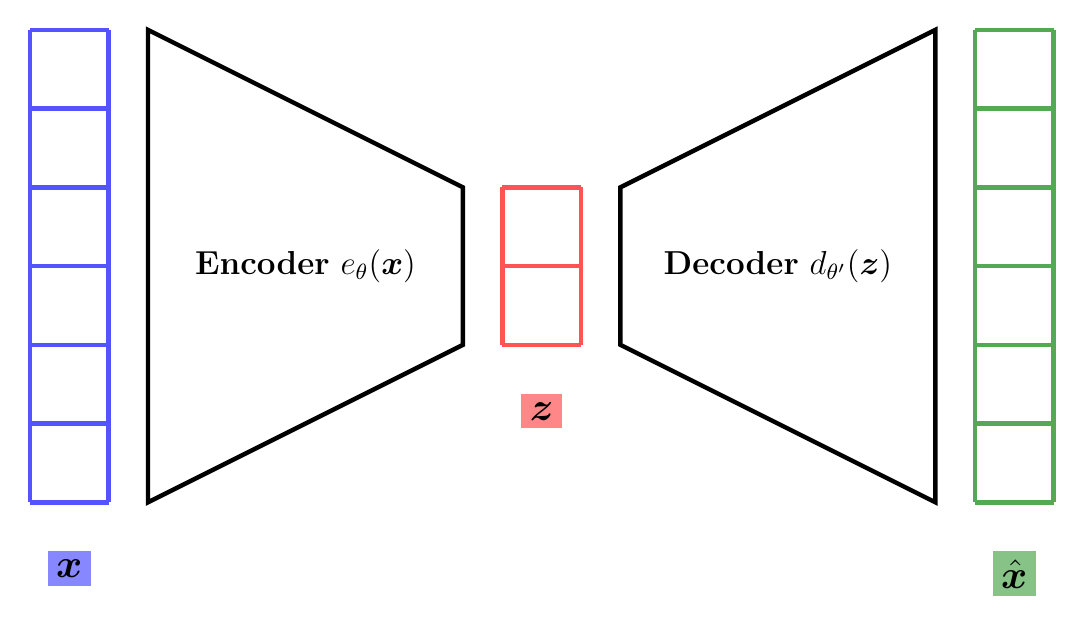
\begin{tikzpicture}
    % \draw[help lines, step=1] (-7, -4) grid (6, 4);

    \draw[step=1, ultra thick, draw=blue!67] (-7, -3) grid (-6, 3);

    \draw[step=1, ultra thick, draw=Green!67] (5, -3) grid (6, 3);

    \draw[step=1, ultra thick, draw=red!67] (-1, -1) grid (0, 1);

    \draw[ultra thick] (-5.5, -3) -- (-1.5, -1) -- (-1.5, 1) -- (-5.5, 3) -- cycle;

    \draw[ultra thick] (4.5, -3) -- (0.5, -1) -- (0.5, 1) -- (4.5, 3) -- cycle;

    \node[anchor=north] at (-6.5, -3.5) {\highlightdark{blue}{\Large $\bm{x}$}};
    \node[anchor=north] at (-0.5, -1.5) {\highlightdark{red}{\Large $\bm{z}$}};
    \node[anchor=north] at (5.5, -3.5) {\highlightdark{Green}{\Large $\hat{\bm{x}}$}};

    \node[] at (-3.5, 0) {\large \textbf{Encoder} $e_{\theta}(\bm{x})$};
    \node[] at (2.5, 0) {\large \textbf{Decoder} $d_{\theta^{\prime}}(\bm{z})$};

  \end{tikzpicture}

  \vspace{-1.5cm}
\end{frame}

\begin{frame}
  \vfill
  {
  \Large
  \[
    \min_{\theta, \theta^{\prime}} \ \sum_{i=1}^N \| \tikzmarknode{a} {\highlightdark{blue}{$\bm{x}_i$}} - \tikzmarknode{c} {\highlightdark{Green}{$( d_{\theta^{\prime}} \circ$ {\highlightdark{red}{$e_{\theta} )(\bm{x}_i)$}}}} \|_2^2
  \]
  }
  \begin{tikzpicture}[overlay, remember picture, >=stealth, nodes={align=left, inner ysep=1pt}, <-]

    \path (a.south) ++ (0, -2em) node[anchor=north east, color=blue!67] (data){Ground truth};
    \draw [color=blue!87] (a.south) |- ([xshift=-0.3ex, color=blue] data.south west);

    \path (c.north) ++ (0, 2em) node[anchor=south west, color=Green!67] (estimate){Estimate};
    \draw [color=Green!87] (c.north) |- ([xshift=0.3ex, color=Green] estimate.south east);

  \end{tikzpicture}

  \vfill
\end{frame}

\begin{frame}
  \vfill

  \begin{overprint}
    \onslide<1>
    \Large
    \[
    \begin{aligned}
      \minimize_{\bm{P}, \bm{Q}} & \quad \sum_{i=1}^N \| \bm{x}_i - \bm{PQ}^T \bm{x}_i \|_2^2 \\
      \subto & \quad \mathrm{rank~} \bm{P} = \mathrm{rank~} \bm{Q} = r
    \end{aligned}
    \]

    \onslide<2>
    \Large
    \[
    \begin{aligned}
      \minimize_{\bm{P}} & \quad \sum_{i=1}^N \| \bm{x}_i - \bm{PP}^T \bm{x}_i \|_2^2 \\
      \subto & \quad \mathrm{rank~} \bm{P} = r
    \end{aligned}
    \]

  \end{overprint}

  \vfill
\end{frame}

\begin{frame}
  \vfill
  \Large
  \[
  \begin{aligned}
    \minimize_{\bm{P}} & \quad \| \bm{X} - \bm{PP}^T \bm{X} \|_F^2 \\
    \subto & \quad \bm{P}^T \bm{P} = \bm{I}_r
  \end{aligned}
  \]

  \vfill
\end{frame}

\begin{frame}
  \vfill

  \begin{tcolorbox}[
    enhanced,
    coltitle=black,
    coltext=white,
    colback=black,
    title=\textbf{Proper Orthogonal Decomposition},
    frame style tile={width=\paperwidth}{background.jpg}
    ]

    \medskip

    \large

    \[
    \bm{P} \boldsymbol{\Lambda} = \bm{C}_{\bm{xx}} \bm{P}
    \]

    \medskip
  \end{tcolorbox}

  \vfill

  $\bm{P}$ corresponds to the left singular vectors of $\bm{X}$.
  The latent representation is given by $\bm{z}_i = \bm{P}^T \bm{x}_i$.
  The optimal rank of the model can be inferred from the distribution of the PCA eigenvalues $\boldsymbol{\Lambda} = \boldsymbol{\Sigma}^2$.

  \vfill
\end{frame}


{
\setbeamercolor*{background canvas}{bg=white}
\setbeamercolor{normal text}{fg=black}
\usebeamercolor[fg]{normal text}

\begin{frame}
  \vfill

  \begin{minipage}{.58\textwidth}
    \centering
    \includegraphics[height=.95\textheight]{leading_eigenfaces}
  \end{minipage}%
  \hfill
  \begin{minipage}{.38\textwidth}
    \textcolor{black}{
    The whole dataset can be correctly approximated using only 500 so-called eigenfaces.
    }
  \end{minipage}
  \vfill
\end{frame}

}
\begin{frame}{Shear-driven cavity POD modes}
  Add POD modes
\end{frame}

\begin{frame}{Shear-driven cavity POD modes}
  Add phase portraits
\end{frame}

{
\setbeamercolor*{background canvas}{bg=white}

\begin{frame}
  \textcolor{black}{Add cylinder flow and pressure coefficient}
\end{frame}

}

\begin{frame}%{Encoder-Decoder network}
  \centering

  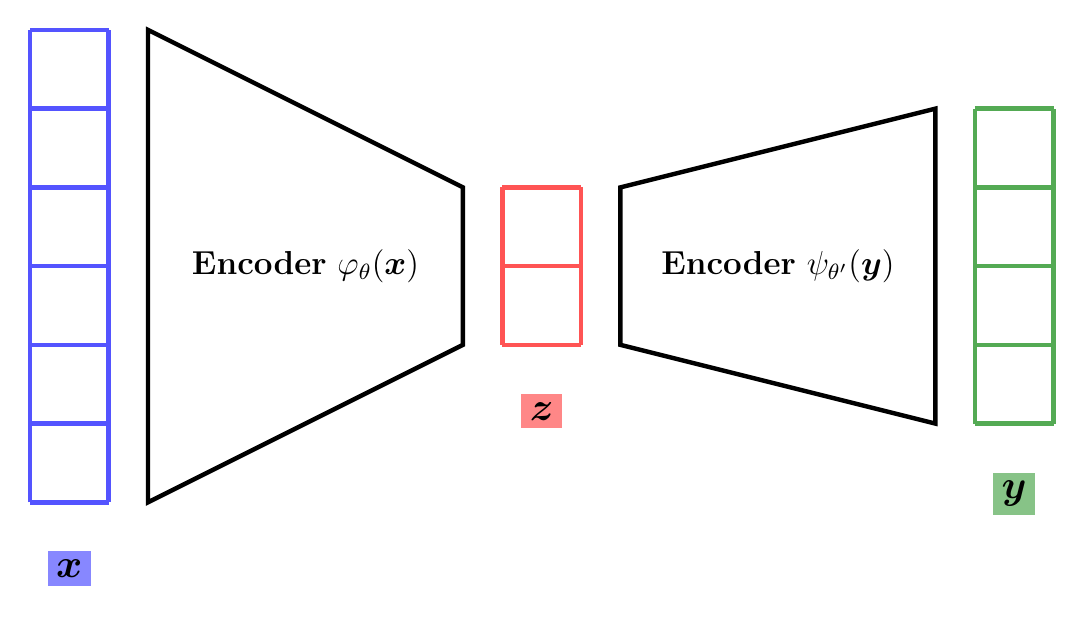
\begin{tikzpicture}
    % \draw[help lines, step=1] (-7, -4) grid (6, 4);

    \draw[step=1, ultra thick, draw=blue!67] (-7, -3) grid (-6, 3);

    \draw[step=1, ultra thick, draw=Green!67] (5, -2) grid (6, 2);

    \draw[step=1, ultra thick, draw=red!67] (-1, -1) grid (0, 1);

    \draw[ultra thick] (-5.5, -3) -- (-1.5, -1) -- (-1.5, 1) -- (-5.5, 3) -- cycle;

    \draw[ultra thick] (4.5, -2) -- (0.5, -1) -- (0.5, 1) -- (4.5, 2) -- cycle;

    \node[anchor=north] at (-6.5, -3.5) {\highlightdark{blue}{\Large $\bm{x}$}};
    \node[anchor=north] at (-0.5, -1.5) {\highlightdark{red}{\Large $\bm{z}$}};
    \node[anchor=north] at (5.5, -2.5) {\highlightdark{Green}{\Large $\bm{y}$}};

    \node[] at (-3.5, 0) {\large \textbf{Encoder} $\varphi_{\theta}(\bm{x})$};
    \node[] at (2.5, 0) {\large \textbf{Encoder} $\psi_{\theta^{\prime}}(\bm{y})$};

  \end{tikzpicture}

  \vspace{-1.5cm}
\end{frame}

\begin{frame}
  \vfill

  \Large
  \[
  \min_{\theta, \theta^{\prime}} \quad \sum_{i=1}^N \| \varphi_{\theta}(\bm{x}_i) - \psi_{\theta^{\prime}}(\bm{y}_i) \|_2^2
  \]

  \vfill
\end{frame}

\begin{frame}
  \vfill
  \Large

  \[
  \begin{aligned}
    \minimize_{\bm{P}, \bm{Q}} & \quad \sum_{i=1}^N \| \bm{P}^T \bm{y}_i - \bm{Q}^T \bm{x}_i \|_2^2 \\
    \subto & \quad \mathrm{rank~} \bm{P} = \mathrm{rank~} \bm{Q} = r
  \end{aligned}
  \]
  \vfill
\end{frame}

\begin{frame}
  \vfill
  \Large
  \[
  \begin{aligned}
    \minimize_{\bm{P}, \bm{Q}} & \quad \| \bm{P}^T \bm{Y} - \bm{Q}^T \bm{X} \|_F^2 \\
    \subto & \quad \bm{P}^T \bm{C}_{yy} \bm{P} = \bm{Q}^T \bm{C}_{xx} \bm{Q} = \bm{I}_r
  \end{aligned}
  \]
  \vfill
\end{frame}

\begin{frame}

  \vfill

    \begin{tcolorbox}[
      enhanced,
      coltitle=black,
      coltext=white,
      colback=black,
      title=\textbf{Canonical Correlation Analysis},
      frame style tile={width=\paperwidth}{background.jpg}
      ]

      \medskip

      \Large

      \[
      \begin{bmatrix}
        \bm{C}_{yy} & \bm{0} \\
        \bm{0} & \bm{C}_{xx}
      \end{bmatrix}
      \begin{bmatrix}
        \bm{P} \\ \bm{Q}
      \end{bmatrix}
      \boldsymbol{\Sigma}
      =
      \begin{bmatrix}
        \bm{0} & \bm{C}_{yx} \\
        \bm{C}_{xy} & \bm{0}
      \end{bmatrix}
      \begin{bmatrix}
        \bm{P} \\ \bm{Q}
      \end{bmatrix}
      \]

      \medskip
    \end{tcolorbox}

    \vfill

    CCA relies on a \emph{generalized eigenproblem}.
    $\bm{P}$ and $\bm{Q}$ describe the encoders such that the latent representations $\bm{z} = \bm{Q}^T \bm{x}$ and $\bm{z}^{\prime} = \bm{P}^T \bm{Y}$ are as similar as possible.
    It is closely related to the concept of \emph{mutual information}.

    \vfill
\end{frame}

{
\setbeamercolor*{background canvas}{bg=white}

\begin{frame}
  \textcolor{black}{Add cylinder flow and pressure coefficient}
\end{frame}

}


\begin{frame}
  \vfill

  \begin{minipage}{.68\textwidth}
    \begin{itemize}
      \item Relies on extremely efficient numerical linear algebra techniques.

      \bigskip

      \item The singular value distribution provides a simple diagnostic to estimate the dimensional of the embedding Euclidean space.

      \bigskip

      \item Component analysis is well understood from a statistical point of view and benefits from good properties.

    \end{itemize}
  \end{minipage}%
  \hfill
  \begin{minipage}{.28\textwidth}
    \centering
    \Huge
    \[
    \color{Green} \bm{+}
    \]
  \end{minipage}

  \vfill
\end{frame}


\begin{frame}
  \vfill

  \begin{minipage}{.68\textwidth}
    \begin{itemize}
      \item The dimension inferred from the singular value distribution tends to over-estimate the intrinsic dimension of the underlying low-dimensional manifold.

      \bigskip

      \item This is directly related to the fact the linear dimensionality reduction techniques do not account for \emph{nonlinear correlations}, only linear ones..

    \end{itemize}
  \end{minipage}%
  \hfill
  \begin{minipage}{.28\textwidth}
    \centering
    \Huge
    \[
    \color{red} \bm{-}
    \]
  \end{minipage}

  \vfill
\end{frame}


\section{Optimal sensor placement}
\begin{frame}
  \sectionpage
\end{frame}

\begin{frame}
  \centering
  \vfill
  \includegraphics[width=\textwidth]{dns_snapshot}
  \vfill
\end{frame}

\begin{frame}
  \vfill

  {
  \Large
  \[
  \tikzmarknode{a} {\highlightdark{blue}{$\bm{y}$}}
  =
  \tikzmarknode{b} {\highlightdark{red}{$\bm{C}$}}
  \tikzmarknode{c} {\highlightdark{Green}{$\bm{x}$}}
  \]
  }

  \begin{tikzpicture}[overlay, remember picture, >=stealth, nodes={align=left, inner ysep=1pt}, <-]

    \path (a.south) ++ (0, -2em) node[anchor=north east, color=blue!67] (data){Observations};
    \draw [color=blue!87] (a.south) |- ([xshift=-0.3ex, color=blue] data.south west);

    \path (b.north) ++ (0, 2em) node[anchor=south west, color=red!67] (obs){Measurement operator};
    \draw [color=red!87] (b.north) |- ([xshift=0.3ex, color=red] obs.south east);

    \path (c.north) ++ (0, -2em) node[anchor=north west, color=Green!67] (estimate){Full state};
    \draw [color=Green!87] (c.south) |- ([xshift=-0.3ex, color=Green] estimate.south east);

  \end{tikzpicture}

  \vfill
\end{frame}

{
\setbeamercolor*{background canvas}{bg=white}

\begin{frame}
  \vfill
  \centering

  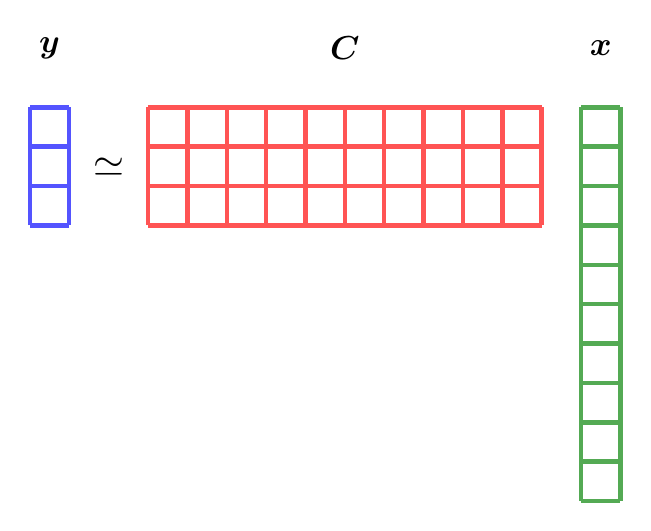
\begin{tikzpicture}
    %\draw[help lines, step=1] (-7, -4) grid (6, 4);

    \draw[step=0.5, ultra thick, draw=blue!67] (-7, -1) grid (-6.5, 0.5);

    \node[anchor=south] at (-6, -0.5) {\Large \textcolor{black}{$\simeq$}};

    \draw[step=0.5, ultra thick, draw=red!67] (-5.5, -1) grid (-0.5, 0.5);

    \draw[step=0.5, ultra thick, draw=Green!67] (0, 0.5) grid (0.5, -4.5);

    \node[text centered] at (-6.75, 1.25) {\large \textcolor{black}{$\bm{y}$}};
    \node[text centered] at (-3, 1.25) {\large \textcolor{black}{$\bm{C}$}};
    \node[text centered] at (0.25, 1.25) {\large \textcolor{black}{$\bm{x}$}};

    % \draw[draw=red, fill=black, ultra thick] (-5.5, -1) rectangle (-5, -0.5);
    % \draw[draw=red, fill=black, ultra thick] (-1.5, -.5) rectangle (-1, 0);
    % \draw[draw=red, fill=black, ultra thick] (-3.5, 0) rectangle (-3, 0.5);

  \end{tikzpicture}

  \vfill
\end{frame}

\begin{frame}
  \vfill
  \centering

  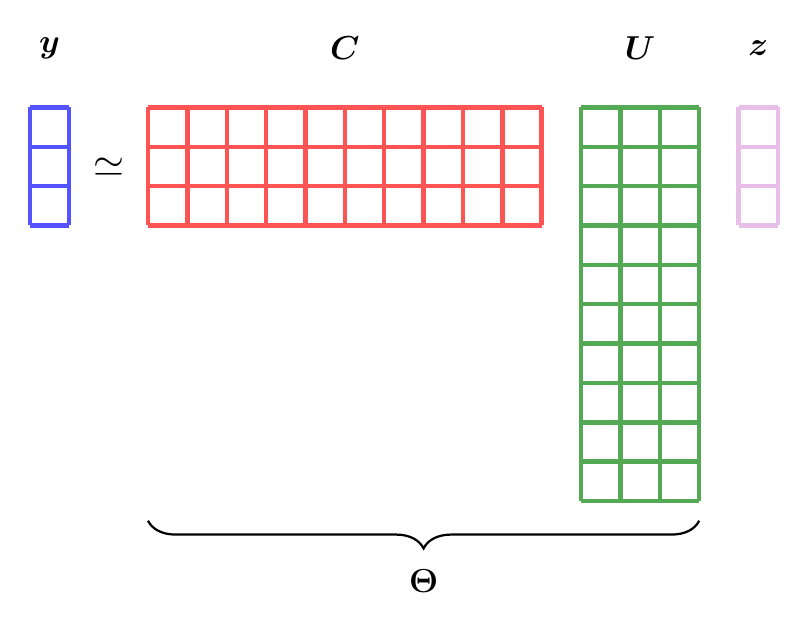
\begin{tikzpicture}
    %\draw[help lines, step=1] (-7, -4) grid (6, 4);

    \draw[step=0.5, ultra thick, draw=blue!67] (-7, -1) grid (-6.5, 0.5);

    \node[anchor=south] at (-6, -0.5) {\Large \textcolor{black}{$\simeq$}};

    \draw[step=0.5, ultra thick, draw=red!67] (-5.5, -1) grid (-0.5, 0.5);

    \draw[step=0.5, ultra thick, draw=Green!67] (0, 0.5) grid (1.5, -4.5);

    \draw[step=0.5, ultra thick, draw=Plum!67] (2, -1) grid (2.5, 0.5);
    \draw[ultra thick, Plum!67] (2, 0.5) -- (2, -1);

    \node[text centered] at (-6.75, 1.25) {\large \textcolor{black}{$\bm{y}$}};
    \node[text centered] at (-3, 1.25) {\large \textcolor{black}{$\bm{C}$}};
    \node[text centered] at (0.75, 1.25) {\large \textcolor{black}{$\bm{U}$}};
    \node[text centered] at (2.25, 1.25) {\large \textcolor{black}{$\bm{z}$}};

    % \draw[draw=red, fill=black, ultra thick] (-5.5, -1) rectangle (-5, -0.5);
    % \draw[draw=red, fill=black, ultra thick] (-1.5, -.5) rectangle (-1, 0);
    % \draw[draw=red, fill=black, ultra thick] (-3.5, 0) rectangle (-3, 0.5);

    \draw [decorate, thick, black, decoration={brace, mirror, amplitude=10pt}] (-5.5, -4.75) -- (1.5, -4.75);
    \node [black, below] at (-2, -5.25) {\large $\boldsymbol{\Theta}$};
  \end{tikzpicture}

  \vfill
\end{frame}

\begin{frame}
  \vfill
  \centering

  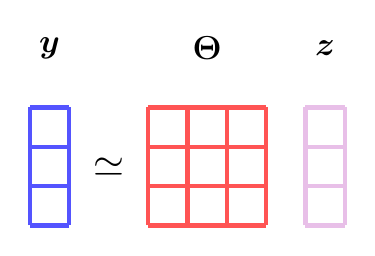
\begin{tikzpicture}
    %\draw[help lines, step=1] (-7, -4) grid (6, 4);

    \draw[step=0.5, ultra thick, draw=blue!67] (-7, -1) grid (-6.5, 0.5);

    \node[anchor=south] at (-6, -0.5) {\Large \textcolor{black}{$\simeq$}};

    \draw[step=0.5, ultra thick, draw=red!67] (-5.5, -1) grid (-4, 0.5);

    \draw[step=0.5, ultra thick, draw=Plum!67] (-3.5, -1) grid (-3, 0.5);
    % \draw[ultra thick, Plum!67] (2, 0.5) -- (2, -1);

    \node[text centered] at (-6.75, 1.25) {\large \textcolor{black}{$\bm{y}$}};
    \node[text centered] at (-4.75, 1.25) {\large \textcolor{black}{$\boldsymbol{\Theta}$}};
    \node[text centered] at (-3.25, 1.25) {\large \textcolor{black}{$\bm{z}$}};

  \end{tikzpicture}

  \vfill
\end{frame}

}

\begin{frame}
  \vfill

  \Large

  \[
  \minimize_{\bm{z}} \quad \| \bm{y}  - \boldsymbol{\Theta} \bm{z} \|_2
  \]

  \vfill
\end{frame}


\begin{frame}
  \vfill

  \Large

  \[
  \bm{z} = \boldsymbol{\Theta}^{-1} \bm{y}
  \]

  \vfill
\end{frame}

\begin{frame}
  \vfill

  \Large
  \[
  \maximize_{\bm{C}} \quad \vert \det(\bm{CU}) \vert
  \]

  \vfill
\end{frame}


\begin{frame}
  \vfill

  \Large
  \[
  \begin{aligned}
    \maximize_{\bm{C}} \quad & \vert \det(\bm{CU}) \vert \\
    \subto \quad & \bm{C}_i \in \left\{ \bm{e}_j \right\}_{j=1, n}
  \end{aligned}
  \]

  \vfill
\end{frame}

\begin{frame}
  \vfill

  {
  \Large

  \[
  \tikzmarknode{a} {\highlightdark{blue}{$\bm{U}$}}^T \tikzmarknode{b} {\highlightdark{red}{$\bm{P}$}} = \bm{Q} \tikzmarknode{c} {\highlightdark{Green}{$\bm{R}$}}
  \]
  }

  \begin{tikzpicture}[overlay, remember picture, >=stealth, nodes={align=left, inner ysep=1pt}, <-]

    \path (a.south) ++ (0, -2em) node[anchor=north east, color=blue!67] (data){Low-rank basis};
    \draw [color=blue!87] (a.south) |- ([xshift=-0.3ex, color=blue] data.south west);

    \path (b.north) ++ (0, 2em) node[anchor=south west, color=red!67] (obs){Permutation matrix};
    \draw [color=red!87] (b.north) |- ([xshift=0.3ex, color=red] obs.south east);

    \path (c.north) ++ (0, -3em) node[anchor=north west, color=Green!67] (estimate){Upper triangular matrix \\ with $\vert r_{i-1} \vert \geq \vert r_i \vert$};
    \draw [color=Green!87] (c.south) |- ([xshift=-0.3ex, color=Green] estimate.south east);

  \end{tikzpicture}

  \vfill
\end{frame}

{
  \setbeamercolor*{background canvas}{bg=white}

\begin{frame}%{Extended Yale B Face dataset}
  \centering
  \vfill
  \includegraphics[height=.8\textheight]{mean_face_ter}
  \vfill
\end{frame}

}

\begin{frame}{Shear-driven cavity flow}

\end{frame}

\begin{frame}
  \vfill

  \begin{minipage}{.68\textwidth}
    \begin{itemize}
      \item Relies on extremely efficient numerical linear algebra techniques.

      \bigskip

      \item Greedy solution to an otherwise intractable combinatorial problem.

      \bigskip

      \item Relevant in many situations and benefits from good empirical performances.

    \end{itemize}
  \end{minipage}%
  \hfill
  \begin{minipage}{.28\textwidth}
    \centering
    \Huge
    \[
    \color{Green} \bm{+}
    \]
  \end{minipage}

  \vfill
\end{frame}


\begin{frame}
  \vfill

  \begin{minipage}{.68\textwidth}
    \begin{itemize}
      \item No easy way to estimate how far from the optimum the greedy solution is.
    \end{itemize}
  \end{minipage}%
  \hfill
  \begin{minipage}{.28\textwidth}
    \centering
    \Huge
    \[
    \color{red} \bm{-}
    \]
  \end{minipage}

  \vfill
\end{frame}


\section{State estimation and low-rank sensing}
\begin{frame}
  \sectionpage
\end{frame}


\begin{frame}
  \vfill

  {
  \Large
  \[
  \tikzmarknode{a} {\highlightdark{blue}{$\bm{y}$}}
  =
  \tikzmarknode{b} {\highlightdark{red}{$\bm{C}$}}
  \tikzmarknode{c} {\highlightdark{Green}{$\bm{x}$}}
  \]
  }

  \begin{tikzpicture}[overlay, remember picture, >=stealth, nodes={align=left, inner ysep=1pt}, <-]

    \path (a.south) ++ (0, -2em) node[anchor=north east, color=blue!67] (data){Observations};
    \draw [color=blue!87] (a.south) |- ([xshift=-0.3ex, color=blue] data.south west);

    \path (b.north) ++ (0, 2em) node[anchor=south west, color=red!67] (obs){Measurement operator};
    \draw [color=red!87] (b.north) |- ([xshift=0.3ex, color=red] obs.south east);

    \path (c.north) ++ (0, -2em) node[anchor=north west, color=Green!67] (estimate){Full state};
    \draw [color=Green!87] (c.south) |- ([xshift=-0.3ex, color=Green] estimate.south east);

  \end{tikzpicture}

  \vfill
\end{frame}

{
\setbeamercolor*{background canvas}{bg=white}

\begin{frame}
  \vfill
  \centering

  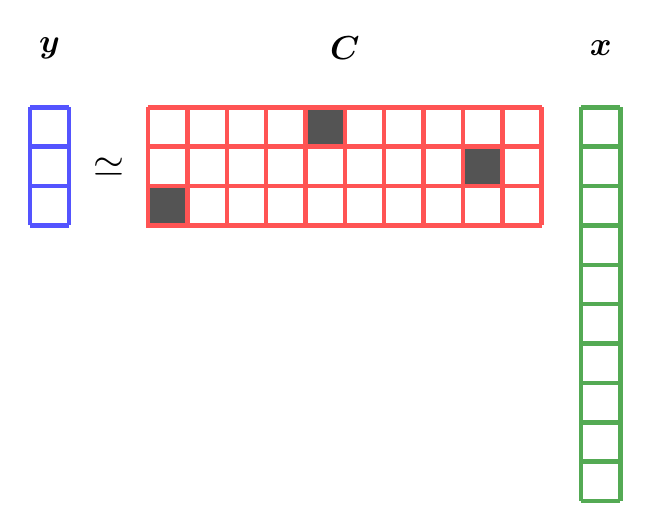
\begin{tikzpicture}
    %\draw[help lines, step=1] (-7, -4) grid (6, 4);

    \draw[step=0.5, ultra thick, draw=blue!67] (-7, -1) grid (-6.5, 0.5);

    \node[anchor=south] at (-6, -0.5) {\Large \textcolor{black}{$\simeq$}};

    \draw[step=0.5, ultra thick, draw=red!67] (-5.5, -1) grid (-0.5, 0.5);

    \draw[step=0.5, ultra thick, draw=Green!67] (0, 0.5) grid (0.5, -4.5);

    \node[text centered] at (-6.75, 1.25) {\large \textcolor{black}{$\bm{y}$}};
    \node[text centered] at (-3, 1.25) {\large \textcolor{black}{$\bm{C}$}};
    \node[text centered] at (0.25, 1.25) {\large \textcolor{black}{$\bm{x}$}};

    \draw[draw=red!67, fill=black!67, ultra thick] (-5.5, -1) rectangle (-5, -0.5);
    \draw[draw=red!67, fill=black!67, ultra thick] (-1.5, -.5) rectangle (-1, 0);
    \draw[draw=red!67, fill=black!67, ultra thick] (-3.5, 0) rectangle (-3, 0.5);

  \end{tikzpicture}

  \vfill
\end{frame}

\begin{frame}
  \vfill
  \centering

  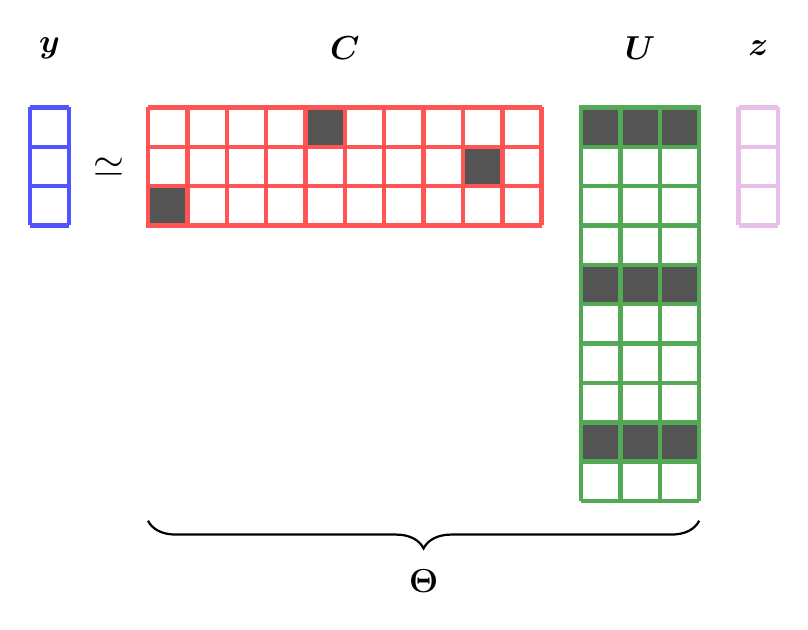
\begin{tikzpicture}
    % \draw[help lines, step=1, black] (-7, -4) grid (6, 4);

    \draw[step=0.5, ultra thick, draw=blue!67] (-7, -1) grid (-6.5, 0.5);

    \node[anchor=south] at (-6, -0.5) {\Large \textcolor{black}{$\simeq$}};

    \draw[step=0.5, ultra thick, draw=red!67] (-5.5, -1) grid (-0.5, 0.5);

    \draw[step=0.5, ultra thick, draw=Green!67] (0, 0.5) grid (1.5, -4.5);

    \draw[step=0.5, ultra thick, draw=Plum!67] (2, 0.5) grid (2.5, -1);
    \draw[ultra thick, Plum!67] (2, 0.5) -- (2, -1);

    \node[text centered] at (-6.75, 1.25) {\large \textcolor{black}{$\bm{y}$}};
    \node[text centered] at (-3, 1.25) {\large \textcolor{black}{$\bm{C}$}};
    \node[text centered] at (0.75, 1.25) {\large \textcolor{black}{$\bm{U}$}};
    \node[text centered] at (2.25, 1.25) {\large \textcolor{black}{$\bm{z}$}};

    \draw[draw=red!67, fill=black!67, ultra thick] (-5.5, -1) rectangle (-5, -0.5);
    \draw[draw=red!67, fill=black!67, ultra thick] (-1.5, -.5) rectangle (-1, 0);
    \draw[draw=red!67, fill=black!67, ultra thick] (-3.5, 0) rectangle (-3, 0.5);

    \draw[draw=Green!67, fill=black!67, ultra thick] (0, 0.5) rectangle (0.5, 0);
    \draw[draw=Green!67, fill=black!67, ultra thick] (0.5, 0.5) rectangle (1, 0);
    \draw[draw=Green!67, fill=black!67, ultra thick] (1, 0.5) rectangle (1.5, 0);

    \draw[draw=Green!67, fill=black!67, ultra thick] (0, -1.5) rectangle (0.5, -2);
    \draw[draw=Green!67, fill=black!67, ultra thick] (0.5, -1.5) rectangle (1, -2);
    \draw[draw=Green!67, fill=black!67, ultra thick] (1, -1.5) rectangle (1.5, -2);

    \draw[draw=Green!67, fill=black!67, ultra thick] (0, -3.5) rectangle (0.5, -4);
    \draw[draw=Green!67, fill=black!67, ultra thick] (0.5, -3.5) rectangle (1, -4);
    \draw[draw=Green!67, fill=black!67, ultra thick] (1, -3.5) rectangle (1.5, -4);


    \draw [decorate, thick, black, decoration={brace, mirror, amplitude=10pt}] (-5.5, -4.75) -- (1.5, -4.75);
    \node [black, below] at (-2, -5.25) {\large $\boldsymbol{\Theta}$};
  \end{tikzpicture}

  \vfill
\end{frame}


\begin{frame}
  \vfill
  \centering

  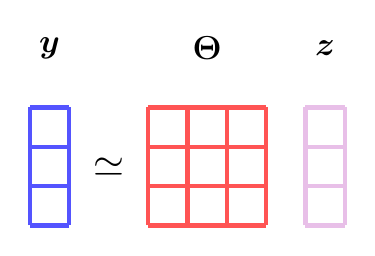
\begin{tikzpicture}
    %\draw[help lines, step=1] (-7, -4) grid (6, 4);

    \draw[step=0.5, ultra thick, draw=blue!67] (-7, -1) grid (-6.5, 0.5);

    \node[anchor=south] at (-6, -0.5) {\Large \textcolor{black}{$\simeq$}};

    \draw[step=0.5, ultra thick, draw=red!67] (-5.5, -1) grid (-4, 0.5);

    \draw[step=0.5, ultra thick, draw=Plum!67] (-3.5, -1) grid (-3, 0.5);
    % \draw[ultra thick, Plum!67] (2, 0.5) -- (2, -1);

    \node[text centered] at (-6.75, 1.25) {\large \textcolor{black}{$\bm{y}$}};
    \node[text centered] at (-4.75, 1.25) {\large \textcolor{black}{$\boldsymbol{\Theta}$}};
    \node[text centered] at (-3.25, 1.25) {\large \textcolor{black}{$\bm{z}$}};

  \end{tikzpicture}

  \vfill
\end{frame}

}

\begin{frame}
  \vfill
  \begin{minipage}{.48\textwidth}
    \centering
    \underline{\textbf{Underdetermined problem}}
  \end{minipage}%
  \hfill
  \begin{minipage}{.48\textwidth}
    \centering
    \underline{\textbf{Overdetermined problem}}
  \end{minipage}

  \bigskip

  \begin{minipage}{.48\textwidth}
    \large
    \[
    \begin{aligned}
      \minimize_{\bm{z}} & \quad \| \bm{z} \|_2 \\
      \subto & \quad \bm{y} = \boldsymbol{\Theta} \bm{z}
    \end{aligned}
    \]
  \end{minipage}%
  \hfill
  \begin{minipage}{.48\textwidth}
    \large
    \[
    \minimize_{\bm{z}} \quad \| \bm{y} - \boldsymbol{\Theta} \bm{z} \|_2^2
    \]
  \end{minipage}

  \vfill
\end{frame}

\begin{frame}
  \vfill
  \centering
  \underline{\textbf{Regularized problem}}

  %\bigskip

  \large
  \[
  \minimize_{\bm{z}} \quad \| \bm{y} - \boldsymbol{\Theta} \bm{z} \|_2^2 + \lambda \| \bm{z} \|_2^2
  \]
  \vfill
\end{frame}

\begin{frame}
  \vfill
  \centering
  \underline{\textbf{Regularized and constrained problem}}

  %\bigskip

  \large
  \[
  \begin{aligned}
    \minimize_{\bm{z}} & \quad \| \bm{y} - \boldsymbol{\Theta} \bm{z} \|_2^2 + \lambda \| \bm{z} \|_2^2 \\
    \subto & \quad \vert z_i \vert \leq 2 \sigma_i \quad \forall \ i
  \end{aligned}
  \]
  \vfill
\end{frame}

{
\setbeamercolor*{background canvas}{bg=white}

\begin{frame}
  \vfill
  \centering

  \includegraphics[width=\textwidth]{eigenfaces_error_plot}

  \vfill
\end{frame}
}

\begin{frame}
  \vfill

  \begin{minipage}{.68\textwidth}
    \begin{itemize}
      \item Low-rank sensing benefits from strong theoretical guarantees.

      \bigskip

      \item Relies on simple yet efficient numerical procedures, both during the training and deployment stages.

      \bigskip

      \item Requires much less data than naïve deep learning alternatives.

    \end{itemize}
  \end{minipage}%
  \hfill
  \begin{minipage}{.28\textwidth}
    \centering
    \Huge
    \[
    \color{Green} \bm{+}
    \]
  \end{minipage}

  \vfill
\end{frame}


\begin{frame}
  \vfill

  \begin{minipage}{.68\textwidth}
    \begin{itemize}
      \item Data needs to be standardized and characterized by an underlying low-rank structure.

      \bigskip

      \item The state estimator is a \textbf{static map}.
      It does not account for the dynamics (if they exist) of the generating process.

      \bigskip

      \item The measurement equation needs to be (approximately) linear.

    \end{itemize}
  \end{minipage}%
  \hfill
  \begin{minipage}{.28\textwidth}
    \centering
    \Huge
    \[
    \color{red} \bm{-}
    \]
  \end{minipage}

  \vfill
\end{frame}

\section{Low-rank structures and sparse sensing for classification}
\begin{frame}
  \sectionpage
\end{frame}

\begin{frame}
  \vfill
  \begin{minipage}{.58\textwidth}
    \centering
    Is it a cat or a dog ?
  \end{minipage}%
  \hfill
  \begin{minipage}{.38\textwidth}

  \end{minipage}
  \vfill
\end{frame}

{
\setbeamercolor*{background canvas}{bg=white}

\begin{frame}

\end{frame}
}

\begin{frame}
  \vfill

  \begin{minipage}{.58\textwidth}
    \centering
    \underline{\textbf{Linear classifier}}

    \[
    \textrm{sign} \left( \bm{w}^T \bm{x} + b \right)
    =
    \begin{cases}
      1 \quad \textrm{then it is a cat,} \\
      -1 \quad \textrm{otherwise a dog.}
    \end{cases}
    \]
  \end{minipage}%
  \hfill
  \begin{minipage}{.48\textwidth}
  \end{minipage}

  \vfill
\end{frame}

\begin{frame}
  Eigenpets
\end{frame}

{
\setbeamercolor*{background canvas}{bg=white}

\begin{frame}
  Classifier
\end{frame}
}

\begin{frame}
  \vfill
  \begin{minipage}{.48\textwidth}
    $\bm{w} \in \mathbb{R}^{20}$, hence only 20 pixels would be necessary to classify the image.
    But how to choose these most informative pixels ?
  \end{minipage}%
  \hfill
  \begin{minipage}{.48\textwidth}
    \Large
    \[
    \begin{aligned}
      \minimize_{\bm{s}} & \quad \| \bm{s} \|_1 \\
      \subto & \quad \bm{U}^T \bm{s} = \bm{w}
    \end{aligned}
    \]
  \end{minipage}
  \vfill
\end{frame}

{
\setbeamercolor*{background canvas}{bg=white}

\begin{frame}
  Selected pixels
\end{frame}

\begin{frame}
  Density map of selected pixels
\end{frame}

\begin{frame}
  Classifier
\end{frame}

}

\begin{frame}
  \vfill

  \begin{minipage}{.68\textwidth}
    \begin{itemize}
      \item
    \end{itemize}
  \end{minipage}%
  \hfill
  \begin{minipage}{.28\textwidth}
    \centering
    \Huge
    \[
    \color{Green} \bm{+}
    \]
  \end{minipage}

  \vfill
\end{frame}


\begin{frame}
  \vfill

  \begin{minipage}{.68\textwidth}
    \begin{itemize}
      \item
    \end{itemize}
  \end{minipage}%
  \hfill
  \begin{minipage}{.28\textwidth}
    \centering
    \Huge
    \[
    \color{red} \bm{-}
    \]
  \end{minipage}

  \vfill
\end{frame}


% % \section{Reduced-order modeling}
% % \begin{frame}
% %   \sectionpage
% % \end{frame}
% %
% % \begin{frame}
% %   \centering
% %   \vfill
% %   \includegraphics[width=\textwidth]{dns_snapshot}
% %   \vfill
% % \end{frame}
% %
% % {
% %
% % \tikzstyle{block} = [draw, fill=blue!67, rectangle,
% %     minimum height=3em, minimum width=6em]
% % \tikzstyle{sum} = [draw, fill=blue!20, circle, node distance=1cm]
% % \tikzstyle{input} = [coordinate]
% % \tikzstyle{output} = [coordinate]
% %
% % \begin{frame}
% %   \vfill
% %   \centering
% %
% %   % The block diagram code is probably more verbose than necessary
% %   \begin{tikzpicture}[auto, node distance=4cm, >=stealth]
% %
% %     \node[input, name=input] {};
% %
% %       \node [
% %         block,
% %         right of=intput,
% %         label=below:Plant,
% %       ] (system) {
% %             \[
% %             \begin{aligned}
% %               \dot{\bm{x}} & = \bm{f}(\bm{x}, \bm{u}) \\
% %               \bm{y} & = \bm{g}(\bm{x}, \bm{u})
% %             \end{aligned}
% %             \]
% %             };
% %
% %       \node[output, name=output, right of=system] {};
% %
% %       \node [
% %       block,
% %       below of=system,
% %       label=below:Controller,
% %       ] (controller) {
% %         $\bm{u} = \mathcal{K}(\bm{y})$
% %       };
% %
% %       \draw[-] (system.east) -- (output) {} node [midway, above] {$\bm{y}$};
% %
% %       \draw[-stealth] (output.center) |- (controller.east);
% %
% %       \draw[-] (controller.west) -| (input.center) ;
% %
% %       \draw[-stealth] (input) -- (system.west) {} node [midway, above] {$\bm{u}$};
% %
% %
% %       % We start by placing the blocks
% %       % \node [input, name=input] {};
% %       % \node [sum, right of=input] (sum) {};
% %       % \node [block, right of=sum] (controller) {Controller};
% %       % \node [
% %       %   block,
% %       %   right of=controller,
% %       %   pin={[pinstyle]above:Disturbances},
% %       %   node distance=5cm,
% %       %   label=below:Plant,
% %       %   ] (system) {
% %       %         \[
% %       %         \begin{aligned}
% %       %           \dot{\bm{x}} & = \bm{f}(\bm{x}, \bm{u}) \\
% %       %           \bm{y} & = \bm{g}(\bm{x}, \bm{u})
% %       %         \end{aligned}
% %       %         \]
% %       %         };
% %       %
% %       % % We draw an edge between the controller and system block to
% %       % % calculate the coordinate u. We need it to place the measurement block.
% %       % \draw [->] (controller) -- node[name=u] {$u$} (system);
% %       % \node [output, right of=system] (output) {};
% %       % \node [block, below of=u] (measurements) {Measurements};
% %       %
% %       % % Once the nodes are placed, connecting them is easy.
% %       % \draw [draw,->] (input) -- node {$r$} (sum);
% %       % \draw [->] (sum) -- node {$e$} (controller);
% %       % \draw [->] (system) -- node [name=y] {$y$}(output);
% %       % \draw [->] (y) |- (measurements);
% %       % \draw [->] (measurements) -| node[pos=0.99] {$-$}
% %       %     node [near end] {$y_m$} (sum);
% %
% %   \end{tikzpicture}
% %
% % \end{frame}
% % }
% %
% % \begin{frame}
% %   \vfill
% %
% %   {
% %   \Large
% %   \[
% %   \begin{aligned}
% %     \dfrac{\mathrm{d} \bm{x}}{\mathrm{d}t} & = \tikzmarknode{a} {\highlightdark{red}{$\bm{A}$}} \bm{x} + \tikzmarknode{b} {\highlightdark{blue}{$\bm{B}$}} \bm{u} \\
% %     \bm{y} & = \tikzmarknode{c} {\highlightdark{Green}{$\bm{C}$}} \bm{x} + \tikzmarknode{d} {\highlightdark{Plum}{$\bm{D}$}} \bm{u}
% %   \end{aligned}
% %   \]
% %   }
% %
% %   \begin{tikzpicture}[overlay, remember picture, >=stealth, nodes={align=left, inner ysep=1pt}, <-]
% %
% %     \path (a.north) ++ (0, 2em) node[anchor=south east, color=red!67] (dynamics){Natural dynamics};
% %     \draw [color=red!87] (a.north) |- ([xshift=0.3ex, color=blue] dynamics.south west);
% %
% %     \path (b.north) ++ (0, 2em) node[anchor=south west, color=blue!67] (actuators){Actuators};
% %     \draw [color=blue!87] (b.north) |- ([xshift=0.3ex, color=blue] actuators.south east);
% %
% %     \path (c.south) ++ (0, -2em) node[anchor=north east, color=Green!67] (obs){Measurements};
% %     \draw [color=Green!87] (c.south) |- ([xshift=-0.3ex, color=Green] obs.south west);
% %
% %     \path (d.south) ++ (0, -2em) node[anchor=north west, color=Plum!67] (feed){Feedthrough};
% %     \draw [color=Plum!87] (d.south) |- ([xshift=-0.3ex, color=Plum] feed.south east);
% %
% %   \end{tikzpicture}
% %
% %   \vfill
% % \end{frame}
% %
% % \begin{frame}
% %   \vfill
% %   \centering
% %
% %   \underline{\textbf{Controlability Gramian}}
% %
% %   \Large
% %   {
% %     \[
% %     \bm{W}_{\mathcal{C}} = \displaystyle \int_0^{\infty} e^{\tau \bm{A}} \bm{BB}^* e^{\tau \bm{A}^*} \ \mathrm{d}\tau
% %     \]
% %   }
% %
% %   \vfill
% % \end{frame}
% %
% % \begin{frame}
% %   \vfill
% %   \centering
% %
% %   \underline{\textbf{Observability Gramian}}
% %
% %   \Large
% %   {
% %     \[
% %     \bm{W}_{\mathcal{O}} = \displaystyle \int_0^{\infty} e^{\tau \bm{A}^*} \bm{C}^* \bm{C} e^{\tau \bm{A}} \ \mathrm{d}\tau
% %     \]
% %   }
% %
% %   \vfill
% % \end{frame}
% %
% %
% % \begin{frame}
% %   \vfill
% %
% %   \begin{tcolorbox}[
% %     enhanced,
% %     coltitle=black,
% %     coltext=white,
% %     colback=black,
% %     title=\textbf{Balancing transform / Balanced tuncation},
% %     frame style tile={width=\paperwidth}{background.jpg}
% %     ]
% %
% %     \medskip
% %     \Large
% %
% %     \[
% %     \begin{bmatrix}
% %       \bm{0} & \bm{I} \\
% %       \bm{I} & \bm{0}
% %     \end{bmatrix}
% %     \begin{bmatrix}
% %       \bm{P} \\ \bm{Q}
% %     \end{bmatrix}
% %     \boldsymbol{\Sigma}
% %       =
% %     \begin{bmatrix}
% %       \bm{W}_{\mathcal{O}} & \bm{0} \\
% %       \bm{0} & \bm{W}_{\mathcal{C}}
% %     \end{bmatrix}
% %     \begin{bmatrix}
% %       \bm{P} \\ \bm{Q}
% %     \end{bmatrix}
% %     \]
% %
% %     \medskip
% %   \end{tcolorbox}
% %
% %   \vfill
% %
% %   BT discards modes which are highly controlable but poorly observable, and vice versa.
% %   The transformed system is \textbf{balanced}.
% %   Its Gramians are given by $\hat{\bm{W}}_{\mathcal{O}} = \hat{\bm{W}}_{\mathcal{C}} = \boldsymbol{\Sigma}$ where $\boldsymbol{\Sigma}$ are the \emph{Hankel singular values} of the system.
% %
% %   \vfill
% % \end{frame}
% %
% % \begin{frame}
% %   \vfill
% %
% %   \centering
% %   \underline{\textbf{Balanced Proper Orthogonal Decomposition}}
% %
% %   \vfill
% %   \begin{overprint}
% %     \onslide<1>
% %     \begin{enumerate}
% %       \item[1.] For each actuator, compute the corresponding impulse reponse
% %       %
% %       \[
% %       \bm{X}_i
% %       =
% %       \begin{bmatrix}
% %         \bm{B}_i & e^{\Delta t \bm{A}} \bm{B}_i & e^{2\Delta t \bm{A}} \bm{B}_i & \cdots & e^{n \Delta t \bm{A}} \bm{B}_i
% %       \end{bmatrix}
% %       \]
% %       %
% %       and assemble the data matrix $\bm{X} = \begin{bmatrix} \bm{X}_1 & \bm{X}_2 & \cdots & \bm{X}_p \end{bmatrix}$.
% %     \end{enumerate}
% %
% %     \onslide<2>
% %     \begin{enumerate}
% %       \item[2.] For each sensor, compute the corresponding \textbf{adjoint} impulse reponse
% %       %
% %       \[
% %       \bm{Y}_i
% %       =
% %       \begin{bmatrix}
% %         \bm{C}^*_i & e^{\Delta t \bm{A}^*} \bm{C}^*_i & e^{2\Delta t \bm{A}^*} \bm{C}^*_i & \cdots & e^{n \Delta t \bm{A}^*} \bm{C}_i^*
% %       \end{bmatrix}
% %       \]
% %       %
% %       and assemble the data matrix $\bm{Y} = \begin{bmatrix} \bm{Y}_1 & \bm{Y}_2 & \cdots & \bm{Y}_q \end{bmatrix}$.
% %     \end{enumerate}
% %
% %     \onslide<3>
% %     \begin{enumerate}
% %       \item[3.] Compute the SVD of $\bm{Y}^T \bm{X}$
% %       %
% %       \[
% %       \bm{Y}^T \bm{X} = \bm{U} \boldsymbol{\Sigma} \bm{V}^T
% %       \]
% %       %
% %       where $\boldsymbol{\Sigma}$ are the \emph{Hankel singular values} of the system.
% %     \end{enumerate}
% %
% %     \onslide<4>
% %     \begin{enumerate}
% %       \item[4.] Compute the first $r$ columns and rows of the balancing transform as
% %       %
% %       \[
% %       \bm{P} = \bm{X} \bm{V} \boldsymbol{\Sigma}^{-\frac12} \quad \text{and} \quad \bm{Q} = \bm{Y} \bm{U} \boldsymbol{\Sigma}^{-\frac12}
% %       \]
% %       %
% %       and proceed with the construction of the reduced-order model.
% %     \end{enumerate}
% %
% %   \end{overprint}
% %
% %   \vfill
% % \end{frame}
% %
% % \begin{frame}
% %   \vfill
% %
% %   \centering
% %   \underline{\textbf{Petrov-Galerkin projection}}
% %
% %   \bigskip
% %
% %   \begin{overprint}
% %     \onslide<1>
% %     \Large
% %     \[
% %     \begin{aligned}
% %       \dfrac{\mathrm{d} \hat{\bm{x}}}{\mathrm{d}t} & = \hat{\bm{A}} \hat{\bm{x}} + \hat{\bm{B}} \bm{u} \\
% %       \hat{\bm{y}} & = \hat{\bm{C}} \hat{\bm{x}} + \hat{\bm{D}} \bm{u}
% %     \end{aligned}
% %     \]
% %
% %     \onslide<2>
% %     \Large
% %     \[\left(
% %     \begin{array}{c|c}
% %       \bm{Q}^T \bm{A} \bm{P} & \bm{Q}^T \bm{B} \\
% %       \hline
% %       \bm{C} \bm{P} & \bm{D}
% %     \end{array}
% %     \right)
% %     \]
% %
% %   \end{overprint}
% %
% %   \vfill
% % \end{frame}
% %
% % \begin{frame}
% %   Example for the shear-driven cavity
% % \end{frame}
%
%
%
%
%
%
%
%
%
%
\section{System identification}
\begin{frame}
  \sectionpage
\end{frame}

\begin{frame}
  \centering
  \vfill
  \includegraphics[width=\textwidth]{dns_snapshot}
  \vfill
\end{frame}

{

\tikzstyle{block} = [draw, fill=blue!67, rectangle,
    minimum height=3em, minimum width=6em]
\tikzstyle{sum} = [draw, fill=blue!20, circle, node distance=1cm]
\tikzstyle{input} = [coordinate]
\tikzstyle{output} = [coordinate]

\begin{frame}
  \vfill
  \centering

  % The block diagram code is probably more verbose than necessary
  \begin{tikzpicture}[auto, node distance=4cm, >=stealth]

    \node[input, name=input] {};

      \node [
        block,
        right of=input,
        label=below:Plant,
      ] (system) {
            \Large
            \textbf{?}
            };

      \node[output, name=output, right of=system] {};

      \node [
      block,
      below of=system,
      label=below:Controller,
      ] (controller) {
        $\bm{u} = \mathcal{K}(\bm{y})$
      };

      \draw[-] (system.east) -- (output) {} node [midway, above] {$\bm{y}$};

      \draw[-stealth] (output.center) |- (controller.east);

      \draw[-] (controller.west) -| (input.center) ;

      \draw[-stealth] (input) -- (system.west) {} node [midway, above] {$\bm{u}$};


      % We start by placing the blocks
      % \node [input, name=input] {};
      % \node [sum, right of=input] (sum) {};
      % \node [block, right of=sum] (controller) {Controller};
      % \node [
      %   block,
      %   right of=controller,
      %   pin={[pinstyle]above:Disturbances},
      %   node distance=5cm,
      %   label=below:Plant,
      %   ] (system) {
      %         \[
      %         \begin{aligned}
      %           \dot{\bm{x}} & = \bm{f}(\bm{x}, \bm{u}) \\
      %           \bm{y} & = \bm{g}(\bm{x}, \bm{u})
      %         \end{aligned}
      %         \]
      %         };
      %
      % % We draw an edge between the controller and system block to
      % % calculate the coordinate u. We need it to place the measurement block.
      % \draw [->] (controller) -- node[name=u] {$u$} (system);
      % \node [output, right of=system] (output) {};
      % \node [block, below of=u] (measurements) {Measurements};
      %
      % % Once the nodes are placed, connecting them is easy.
      % \draw [draw,->] (input) -- node {$r$} (sum);
      % \draw [->] (sum) -- node {$e$} (controller);
      % \draw [->] (system) -- node [name=y] {$y$}(output);
      % \draw [->] (y) |- (measurements);
      % \draw [->] (measurements) -| node[pos=0.99] {$-$}
      %     node [near end] {$y_m$} (sum);

  \end{tikzpicture}

\end{frame}
}

\begin{frame}
  \vfill
  \centering

  \underline{\textbf{Convolution model}}

  \Large
  \[
  \bm{y}_i = \bm{f} \left( \bm{u}_i, \bm{u}_{i-1}, \bm{u}_{i-2}, \cdots \right)
  \]

  \vfill
\end{frame}


\begin{frame}
  \vfill

  {
  \Large
  \[
  \begin{aligned}
    \bm{x}_{i+1} & = \tikzmarknode{a} {\highlightdark{red}{$\bm{A}$}} \bm{x}_i + \tikzmarknode{b} {\highlightdark{blue}{$\bm{B}$}} \bm{u}_i \\
    \bm{y}_{i} & = \tikzmarknode{c} {\highlightdark{Green}{$\bm{C}$}} \bm{x}_i + \tikzmarknode{d} {\highlightdark{Plum}{$\bm{D}$}} \bm{u}_i
  \end{aligned}
  \]
  }

  \begin{tikzpicture}[overlay, remember picture, >=stealth, nodes={align=left, inner ysep=1pt}, <-]

    \path (a.north) ++ (0, 2em) node[anchor=south east, color=red!67] (dynamics){Natural dynamics};
    \draw [color=red!87] (a.north) |- ([xshift=0.3ex, color=blue] dynamics.south west);

    \path (b.north) ++ (0, 2em) node[anchor=south west, color=blue!67] (actuators){Actuators};
    \draw [color=blue!87] (b.north) |- ([xshift=0.3ex, color=blue] actuators.south east);

    \path (c.south) ++ (0, -2em) node[anchor=north east, color=Green!67] (obs){Measurements};
    \draw [color=Green!87] (c.south) |- ([xshift=-0.3ex, color=Green] obs.south west);

    \path (d.south) ++ (0, -2em) node[anchor=north west, color=Plum!67] (feed){Feedthrough};
    \draw [color=Plum!87] (d.south) |- ([xshift=-0.3ex, color=Plum] feed.south east);

  \end{tikzpicture}

  \vfill
\end{frame}

\begin{frame}
  \vfill
  \centering

  \large
  \begin{tabular}{c|r|r}
    Input $\bm{u}_i$ & State $\bm{x}_i$ & Output $\bm{y}_i$ \\
    \hline
    $\bm{u}_0$ & $\bm{0}$ & $\bm{Du}_0$ \\
    $\bm{u}_1$ & $\bm{Bu}_0$ & $\bm{CBu}_0 + \bm{Du}_1$ \\
    $\bm{u}_2$ & $\bm{ABu}_0 + \bm{Bu}_1$ & $\bm{CABu}_0 + \bm{CBu}_1 + \bm{Du}_2$ \\
    $\bm{u}_3$ & $\bm{A}^2 \bm{Bu}_0 + \bm{ABu}_1 + \bm{Bu}_2$ & $\bm{CA}^2 \bm{Bu}_0 + \bm{CABu}_1 + \bm{CBu}_2 + \bm{Du}_3$ \\
    $\vdots$ & $\vdots$ & $\vdots$ \\
    $\bm{u}_k$ & $\displaystyle \sum_{i=1}^k \bm{A}^{k-i} \bm{Bu}_{k-i}$ & $\displaystyle \sum_{i=1}^k \bm{CA}^{k-i} \bm{Bu}_{k-i} + \bm{Du}_k$
  \end{tabular}

  \vfill
\end{frame}

\begin{frame}
  \vfill

    {\Large
    \[
    \tikzmarknode{a}{\highlightdark{red}{$\bm{y}(t)$}} = \tikzmarknode{c}{\highlightdark{Green}{$\bm{h}(t)$}} * \tikzmarknode{b}{\highlightdark{blue}{$\bm{u}(t)$}}
    \]
    }

    \begin{tikzpicture}[overlay, remember picture, >=stealth, nodes={align=left, inner ysep=1pt}, <-]

      \path (a.north) ++ (0, 2em) node[anchor=south east, color=red!67] (U){Output};
      \draw [color=red!87] (a.north) |- ([xshift=0.3ex, color=red] U.south west);

      \path (b.south) ++ (0, -2em) node[anchor=north east, color=blue!67] (Sigma){Input};
      \draw [color=blue!87] (b.south) |- ([xshift=-0.3ex, color=blue] Sigma.south west);

      \path (c.north) ++ (0, 2em) node[anchor=south west, color=OliveGreen!67] (V){Unknown conv. kernel};
      \draw [color=OliveGreen!87] (c.north) |- ([xshift=0.3ex, color=OliveGreen] V.south east);

    \end{tikzpicture}

  \vfill
\end{frame}

\begin{frame}
  \vfill
  \Large
  \[
  \begin{bmatrix}
    \bm{y}_0 \\ \bm{y}_1 \\ \bm{y}_2 \\ \bm{y}_3 \\ \vdots
  \end{bmatrix}
  =
  \begin{bmatrix}
    \bm{u}_0 & \cdots \\
    \bm{u}_1 & \bm{u}_0 & \cdots \\
    \bm{u}_2 & \bm{u}_1 & \bm{u}_0 & \cdots \\
    \bm{u}_3 & \bm{u}_2 & \bm{u}_1 & \bm{u}_0 & \cdots \\
    \vdots & \ddots & \ddots & \ddots & \ddots
  \end{bmatrix}
  \begin{bmatrix}
    \bm{D} \\ \bm{CB} \\ \bm{CAB} \\ \bm{CA}^2 \bm{B} \\ \bm{CA}^3 \bm{B} \\ \vdots
  \end{bmatrix}
  \]
  \vfill
\end{frame}

\begin{frame}
  \vfill

  {\Large
  \[
  \minimize_{\bm{h}} \quad \| \tikzmarknode{a}{\highlightdark{red}{$\bm{y}$}} - \tikzmarknode{b}{\highlightdark{blue}{$\mathcal{T}(\bm{u})$}} \tikzmarknode{c}{\highlightdark{Green}{$\bm{h}$}} \|_p + \mathcal{R}(\bm{h})
  \]
  }

  \begin{tikzpicture}[overlay, remember picture, >=stealth, nodes={align=left, inner ysep=1pt}, <-]

    \path (a.north) ++ (0, 2em) node[anchor=south east, color=red!67] (U){Output sequence};
    \draw [color=red!87] (a.north) |- ([xshift=0.3ex, color=red] U.south west);

    \path (b.south) ++ (0, -2em) node[anchor=north east, color=blue!67] (Sigma){Toeplitz matrix built \\ using the input sequence};
    \draw [color=blue!87] (b.south) |- ([xshift=-0.3ex, color=blue] Sigma.south west);

    \path (c.north) ++ (0, 2em) node[anchor=south west, color=OliveGreen!67] (V){Unknown conv. kernel};
    \draw [color=OliveGreen!87] (c.north) |- ([xshift=0.3ex, color=OliveGreen] V.south east);

  \end{tikzpicture}

  \vfill
\end{frame}

{
\setbeamercolor*{background canvas}{bg=white}
\setbeamercolor{normal text}{fg=black}
\usebeamercolor[fg]{normal text}

\begin{frame}
  \vfill

  \begin{minipage}{.48\textwidth}
    \centering
    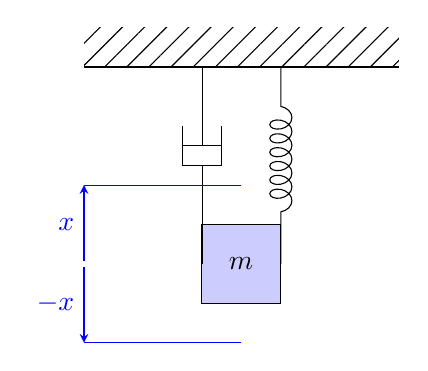
\begin{tikzpicture}[>=stealth]
        \path[pattern={Lines[angle=45,distance={8pt/sqrt(2)}]}] (-2, 5) edge ++(4,0) rectangle ++ (4, 0.5);

        \draw[decorate,decoration={coil, segment length=5pt, aspect=0.7, amplitude=4pt,
            pre=lineto, pre length=5mm, post=lineto, post length=5mm}] (0.5, 5) -- (0.5, 2.5)
        node[left, draw, minimum size=1cm, fill=blue!20] (m) {$m$};

        \draw[] (-0.5, 5) -- (-0.5, 4) {};
        \draw[] (-0.25, 4) -- (-0.75, 4) {};

        \draw[] (-0.5, 3.75) -- (-0.5, 2.5) {};
        \draw[] (-0.25, 3.75) -- (-0.75, 3.75) {};

        \draw[] (-0.25, 3.75) -- (-0.25, 4.25) {};
        \draw[] (-0.75, 3.75) -- (-0.75, 4.25) {};

        \draw[blue] (m.center-|0, 0) ++ (0, 1) -- ++ (-2, 0)
        edge[<-,edge label'=$x$,shorten >=1pt] (m.center-|-2, 0)
        (m.center-|0, 0) ++ (0, -1) -- ++ (-2, 0)
        edge[<-,edge label=$-x$,shorten >=1pt] (m.center-|-2, 0);
        %(m.east) edge[dashed] (m.east-|2, 0);
        %(m.east-|2, 0) node[right] {Equilibrium};
    \end{tikzpicture}
  \end{minipage}%
  \hfill
  \begin{minipage}{.48\textwidth}
    \centering

    \Large
    \[
    \begin{aligned}
      \dfrac{\mathrm{d}}{\mathrm{d}t} \begin{bmatrix} x \\ v \end{bmatrix}
      & =
      \begin{bmatrix}
        0 & 1 \\
        -1 & -2\zeta
      \end{bmatrix}
      \begin{bmatrix} x \\ v \end{bmatrix}
      +
      \begin{bmatrix}
        0 \\ 1
      \end{bmatrix} u \\
      y & = \begin{bmatrix} 1 & 0 \end{bmatrix} \begin{bmatrix} x \\ v \end{bmatrix}
    \end{aligned}
    \]

  \end{minipage}

  \vfill
\end{frame}

\begin{frame}

\end{frame}

}

\begin{frame}
  \vfill

  \begin{minipage}{.68\textwidth}
    \begin{itemize}
      \item Relies on simple linear regression.

      \bigskip

      \item Easy to extend to nonlinear systems (e.g. LSTM)

      \bigskip

      \item Prior knowledge can be included through regularization or constraints.

    \end{itemize}
  \end{minipage}%
  \hfill
  \begin{minipage}{.28\textwidth}
    \centering
    \Huge
    \[
    \color{Green} \bm{+}
    \]
  \end{minipage}

  \vfill
\end{frame}


\begin{frame}
  \vfill

  \begin{minipage}{.68\textwidth}
    \begin{itemize}
      \item The length of the convolution kernel is \emph{a priori} unknown.

      \bigskip

      \item The longer the kernel, the more data is needed to obtain converged estimates.

      \bigskip

      \item It is \emph{a priori} unrelated to the number of degrees of freedom in the system.

    \end{itemize}
  \end{minipage}%
  \hfill
  \begin{minipage}{.28\textwidth}
    \centering
    \Huge
    \[
    \color{red} \bm{-}
    \]
  \end{minipage}

  \vfill
\end{frame}

\begin{frame}
  \vfill

  {
  \Large
  \[
  \begin{aligned}
    \bm{x}_{i+1} & = \tikzmarknode{a} {\highlightdark{red}{$\bm{A}$}} \bm{x}_i + \tikzmarknode{b} {\highlightdark{blue}{$\bm{B}$}} \bm{u}_i \\
    \bm{y}_{i} & = \tikzmarknode{c} {\highlightdark{Green}{$\bm{C}$}} \bm{x}_i + \tikzmarknode{d} {\highlightdark{Plum}{$\bm{D}$}} \bm{u}_i
  \end{aligned}
  \]
  }

  \begin{tikzpicture}[overlay, remember picture, >=stealth, nodes={align=left, inner ysep=1pt}, <-]

    \path (a.north) ++ (0, 2em) node[anchor=south east, color=red!67] (dynamics){Natural dynamics};
    \draw [color=red!87] (a.north) |- ([xshift=0.3ex, color=blue] dynamics.south west);

    \path (b.north) ++ (0, 2em) node[anchor=south west, color=blue!67] (actuators){Actuators};
    \draw [color=blue!87] (b.north) |- ([xshift=0.3ex, color=blue] actuators.south east);

    \path (c.south) ++ (0, -2em) node[anchor=north east, color=Green!67] (obs){Measurements};
    \draw [color=Green!87] (c.south) |- ([xshift=-0.3ex, color=Green] obs.south west);

    \path (d.south) ++ (0, -2em) node[anchor=north west, color=Plum!67] (feed){Feedthrough};
    \draw [color=Plum!87] (d.south) |- ([xshift=-0.3ex, color=Plum] feed.south east);

  \end{tikzpicture}

  \vfill
\end{frame}


\begin{frame}%{Observability and Controlability}
  \vfill

  \begin{minipage}{.28\textwidth}
    \Large

    \[
    \mathcal{O}_k
    =
    \begin{bmatrix}
      \bm{C} \\ \bm{CA} \\ \bm{CA}^2 \\ \bm{CA}^3 \\ \vdots \\ \bm{CA}^{k-1}
    \end{bmatrix}
    \]
  \end{minipage}%
  \hfill
  \begin{minipage}{.68\textwidth}
    \Large

    \[
    \mathcal{C}_k
    =
    \begin{bmatrix}
      \bm{B} & \bm{AB} & \bm{A}^2 \bm{B} & \bm{A}^3 \bm{B} & \cdots & \bm{A}^{k-1} \bm{B}
    \end{bmatrix}
    \]
  \end{minipage}

  \vfill

  \begin{minipage}{.28\textwidth}
    \centering
    \underline{\textbf{Observability}}
  \end{minipage}%
  \hfill
  \begin{minipage}{.68\textwidth}
    \centering
    \underline{\textbf{Controlability}}
  \end{minipage}

  \vfill
\end{frame}

\begin{frame}
  \centering
  \vfill

  {\Large
  \[
    \bm{h}_k
    =
    \begin{bmatrix}
      \bm{D} & \bm{CB} & \bm{CAB} & \bm{CA}^2\bm{B} & \bm{CA}^3 \bm{B} & \cdots & \bm{CA}^{k-1} \bm{B}
    \end{bmatrix}
  \]
  }

  \bigskip

  \underline{\textbf{Markov parameters of the system}}

  \vfill
\end{frame}


% {
% \setbeamercolor*{background canvas}{bg=white}
% \setbeamercolor{normal text}{fg=black}
% \usebeamercolor[fg]{normal text}
%
% \begin{frame}
%   \vfill
%
%   \begin{minipage}{.48\textwidth}
%     \centering
%     \begin{tikzpicture}[>=stealth]
%         \path[pattern={Lines[angle=45,distance={8pt/sqrt(2)}]}] (-2, 5) edge ++(4,0) rectangle ++ (4, 0.5);
%
%         \draw[decorate,decoration={coil, segment length=5pt, aspect=0.7, amplitude=4pt,
%             pre=lineto, pre length=5mm, post=lineto, post length=5mm}] (0.5, 5) -- (0.5, 2.5)
%         node[left, draw, minimum size=1cm, fill=blue!20] (m) {$m$};
%
%         \draw[] (-0.5, 5) -- (-0.5, 4) {};
%         \draw[] (-0.25, 4) -- (-0.75, 4) {};
%
%         \draw[] (-0.5, 3.75) -- (-0.5, 2.5) {};
%         \draw[] (-0.25, 3.75) -- (-0.75, 3.75) {};
%
%         \draw[] (-0.25, 3.75) -- (-0.25, 4.25) {};
%         \draw[] (-0.75, 3.75) -- (-0.75, 4.25) {};
%
%         \draw[blue] (m.center-|0, 0) ++ (0, 1) -- ++ (-2, 0)
%         edge[<-,edge label'=$x$,shorten >=1pt] (m.center-|-2, 0)
%         (m.center-|0, 0) ++ (0, -1) -- ++ (-2, 0)
%         edge[<-,edge label=$-x$,shorten >=1pt] (m.center-|-2, 0);
%         %(m.east) edge[dashed] (m.east-|2, 0);
%         %(m.east-|2, 0) node[right] {Equilibrium};
%     \end{tikzpicture}
%   \end{minipage}%
%   \hfill
%   \begin{minipage}{.48\textwidth}
%     \centering
%
%     \Large
%     \[
%     \begin{aligned}
%       \dfrac{\mathrm{d}}{\mathrm{d}t} \begin{bmatrix} x \\ v \end{bmatrix}
%       & =
%       \begin{bmatrix}
%         0 & 1 \\
%         -1 & -2\zeta
%       \end{bmatrix}
%       \begin{bmatrix} x \\ v \end{bmatrix}
%       +
%       \begin{bmatrix}
%         0 \\ 1
%       \end{bmatrix} u \\
%       y & = \begin{bmatrix} 1 & 0 \end{bmatrix} \begin{bmatrix} x \\ v \end{bmatrix}
%     \end{aligned}
%     \]
%
%   \end{minipage}
%
%   \vfill
% \end{frame}
%
% \begin{frame}
%   \vfill
%   \centering
%   \includegraphics[width=\textwidth]{pendulum_impulse_response}
%   \vfill
% \end{frame}
%
% }

\begin{frame}{EigenRealization Algorithm}
  \vfill

  \Large
  \[
  \bm{H}_1
  =
  \begin{bmatrix}
    h_1 & h_2 & h_3 & h_4 & h_5 \\
    h_2 & h_3 & h_4 & h_5 & h_6 \\
    h_3 & h_4 & h_5 & h_6 & h_7 \\
    h_4 & h_5 & h_6 & h_7 & h_8 \\
    h_5 & h_6 & h_7 & h_8 & h_9 \\
  \end{bmatrix}
  \]

  \vfill
\end{frame}

\begin{frame}{EigenRealization Algorithm}
  \vfill

  \Large
  \[
  \bm{H}_1
  =
  \begin{bmatrix}
    \bm{CB} & \bm{CAB} & \bm{CA}^2 \bm{B} & \bm{CA}^3 \bm{B} & \bm{CA}^4 \bm{B} \\
    \bm{CAB} & \bm{CA}^2 \bm{B} & \bm{CA}^3 \bm{B} & \bm{CA}^4 \bm{B} & \bm{CA}^5 \bm{B} \\
    \bm{CA}^2 \bm{B} & \bm{CA}^3 \bm{B} & \bm{CA}^4 \bm{B} & \bm{CA}^5 \bm{B} & \bm{CA}^6 \bm{B} \\
    \bm{CA}^3 \bm{B} & \bm{CA}^4 \bm{B} & \bm{CA}^5 \bm{B} & \bm{CA}^6 \bm{B} & \bm{CA}^7 \bm{B} \\
    \bm{CA}^4 \bm{B} & \bm{CA}^5 \bm{B} & \bm{CA}^6 \bm{B} & \bm{CA}^7 \bm{B} & \bm{CA}^8 \bm{B} \\
  \end{bmatrix}
  \]

  \vfill
\end{frame}


\begin{frame}{EigenRealization Algorithm}
  \vfill

  \Large
  \[
  \bm{H}_1
  =
  \begin{bmatrix}
    \bm{C} \\ \bm{CA} \\ \bm{CA}^2 \\ \bm{CA}^3 \\ \bm{CA}^4
  \end{bmatrix}
  \begin{bmatrix}
    \bm{B} & \bm{AB} & \bm{A}^2 \bm{B} & \bm{A}^3 \bm{B} & \bm{A}^4 \bm{B}
  \end{bmatrix}
  \]

  \vfill
\end{frame}

\begin{frame}{EigenRealization Algorithm}
  \vfill

  \centering

  \underline{\textbf{Observability :}} \quad {\Large \( \mathcal{O} = \bm{U} \boldsymbol{\Sigma}^{\frac12} \)}

  \vfill

  \underline{\textbf{Controlability :}} \quad {\Large \( \mathcal{C} = \boldsymbol{\Sigma}^{\frac12} \bm{V}^T \)}

  \vfill
\end{frame}

\begin{frame}{EigenRealization Algorithm}
  \vfill

  \Large
  \[
  \bm{H}_2
  =
  \begin{bmatrix}
    h_2 & h_3 & h_4 & h_5 & h_6 \\
    h_3 & h_4 & h_5 & h_6 & h_7 \\
    h_4 & h_5 & h_6 & h_7 & h_8 \\
    h_5 & h_6 & h_7 & h_8 & h_9 \\
    h_6 & h_7 & h_8 & h_9 & h_{10} \\
  \end{bmatrix}
  \]

  \vfill
\end{frame}


\begin{frame}{EigenRealization Algorithm}
  \vfill

  \Large
  \[
  \bm{H}_2
  =
  \begin{bmatrix}
    \bm{C} \\ \bm{CA} \\ \bm{CA}^2 \\ \bm{CA}^3 \\ \bm{CA}^4
  \end{bmatrix}
  \bm{A}
  \begin{bmatrix}
    \bm{B} & \bm{AB} & \bm{A}^2 \bm{B} & \bm{A}^3 \bm{B} & \bm{A}^4 \bm{B}
  \end{bmatrix}
  \]

  \vfill
\end{frame}

\begin{frame}{EigenRealization Algorithm}
  \vfill

  \begin{minipage}{.48\textwidth}
    \centering
    \underline{\textbf{Natural dynamics}}
  \end{minipage}%
  \hfill
  \begin{minipage}{.48\textwidth}
    \centering
    \underline{\textbf{Actuators}}
  \end{minipage}

  \bigskip

  \begin{minipage}{.48\textwidth}
    {
    \Large
    \[
      \bm{A} = \mathcal{O}^{\dagger} \bm{H}_2 \mathcal{C}^{\dagger}
    \]
    }
  \end{minipage}%
  \hfill
  \begin{minipage}{.48\textwidth}
    {
    \Large
    \[
      \bm{B} = \left[ \boldsymbol{\Sigma}^{\frac12} \bm{V}^T \right]_{:, 1:p}
    \]
    }
  \end{minipage}

  \vfill

  \begin{minipage}{.48\textwidth}
    \centering
    \underline{\textbf{Measurements}}
  \end{minipage}%
  \hfill
  \begin{minipage}{.48\textwidth}
    \centering
    \underline{\textbf{Feedthrough}}
  \end{minipage}

  \bigskip

  \begin{minipage}{.48\textwidth}
    {
    \Large
    \[
      \bm{C} = \left[ \bm{U} \boldsymbol{\Sigma}^{\frac12} \right]_{1:q, :}
    \]
    }
  \end{minipage}%
  \hfill
  \begin{minipage}{.48\textwidth}
    {
    \Large
    \[
      \bm{D} = \bm{h}_0
    \]
    }
  \end{minipage}

  \vfill
\end{frame}

{
\setbeamercolor*{background canvas}{bg=white}
\setbeamercolor{normal text}{fg=black}
\usebeamercolor[fg]{normal text}

\begin{frame}
  \vfill

  \begin{minipage}{.48\textwidth}
    \centering
    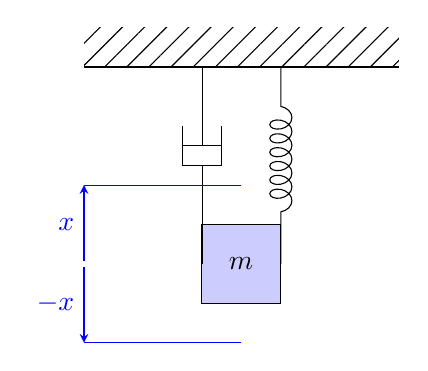
\begin{tikzpicture}[>=stealth]
        \path[pattern={Lines[angle=45,distance={8pt/sqrt(2)}]}] (-2, 5) edge ++(4,0) rectangle ++ (4, 0.5);

        \draw[decorate,decoration={coil, segment length=5pt, aspect=0.7, amplitude=4pt,
            pre=lineto, pre length=5mm, post=lineto, post length=5mm}] (0.5, 5) -- (0.5, 2.5)
        node[left, draw, minimum size=1cm, fill=blue!20] (m) {$m$};

        \draw[] (-0.5, 5) -- (-0.5, 4) {};
        \draw[] (-0.25, 4) -- (-0.75, 4) {};

        \draw[] (-0.5, 3.75) -- (-0.5, 2.5) {};
        \draw[] (-0.25, 3.75) -- (-0.75, 3.75) {};

        \draw[] (-0.25, 3.75) -- (-0.25, 4.25) {};
        \draw[] (-0.75, 3.75) -- (-0.75, 4.25) {};

        \draw[blue] (m.center-|0, 0) ++ (0, 1) -- ++ (-2, 0)
        edge[<-,edge label'=$x$,shorten >=1pt] (m.center-|-2, 0)
        (m.center-|0, 0) ++ (0, -1) -- ++ (-2, 0)
        edge[<-,edge label=$-x$,shorten >=1pt] (m.center-|-2, 0);
        %(m.east) edge[dashed] (m.east-|2, 0);
        %(m.east-|2, 0) node[right] {Equilibrium};
    \end{tikzpicture}
  \end{minipage}%
  \hfill
  \begin{minipage}{.48\textwidth}
    \centering

      \includegraphics[width=.8\textwidth]{Hankel_matrix_pendulum}

      \vfill

      \[
      \boldsymbol{\Sigma}
      =
      \begin{bmatrix}
        27.68 & 22.62 & 0 & 0 & \cdots
      \end{bmatrix}
      \]

  \end{minipage}

  \vfill
\end{frame}

\begin{frame}
  \centering
  \vfill

  \includegraphics[width=\textwidth]{pendulum_identified_response}

  \vfill
\end{frame}

}

\begin{frame}
  Cylinder flow example
\end{frame}


\begin{frame}
  \vfill

  \begin{minipage}{.68\textwidth}
    \begin{itemize}
      \item Relies solely on the impulse response of the system and efficient numerical linear algebra.

      \bigskip

      \item Identifies the minimal number of degrees of freedom needed to represent the dynamics.

      \bigskip

      \item Benefits from strong theoretical guarantees and is well-grounded in control theory.

    \end{itemize}
  \end{minipage}%
  \hfill
  \begin{minipage}{.28\textwidth}
    \centering
    \Huge
    \[
    \color{Green} \bm{+}
    \]
  \end{minipage}

  \vfill
\end{frame}

\begin{frame}
  \vfill

  \begin{minipage}{.68\textwidth}
    \begin{itemize}
      \item Need a really good estimate of the impulse reponse.

      \bigskip

      \item Extension to \textbf{interpretable} nonlinear systems is not straitghtforward.

      \bigskip

      \item Parametric variations can be easily included into this framework.

    \end{itemize}
  \end{minipage}%
  \hfill
  \begin{minipage}{.28\textwidth}
    \centering
    \Huge
    \[
    \color{red} \bm{-}
    \]
  \end{minipage}

  \vfill
\end{frame}


\section{Conclusion}
\begin{frame}
  \sectionpage
\end{frame}

\begin{frame}
  \vfill

  \vfill
\end{frame}

\end{document}
